\section{Methods} \label{sec:methods}

\subsection{The Algorithm} \label{sec:algorithm}

We present a modification of Algorithm~\ref{alg:old} where we replace the best path search in line 9 with more intelligent consolidation step to deal with missing ranks. The main idea of this algorithm is to realize that, as previously stated, once data from a specific rank is no longer included in one organism, it will not be included in any subsequent organisms, meaning that the level in the tree corresponding to that rank is no longer useful. Therefore, we can modify the tree to act as if that level was no longer there, building shortcuts from the previous level to the next used level, and `hiding', yet not entirely removing, all the nodes in the current level (steps 1-2 in Figure~\ref{fig:algo-diagram}). As a result, the children of the removed level now become the children of that level's parent. 

\begin{figure*}
\begin{minipage}{0.74\linewidth}
\centering
\begin{minipage}{0.32\linewidth}
  \centering
  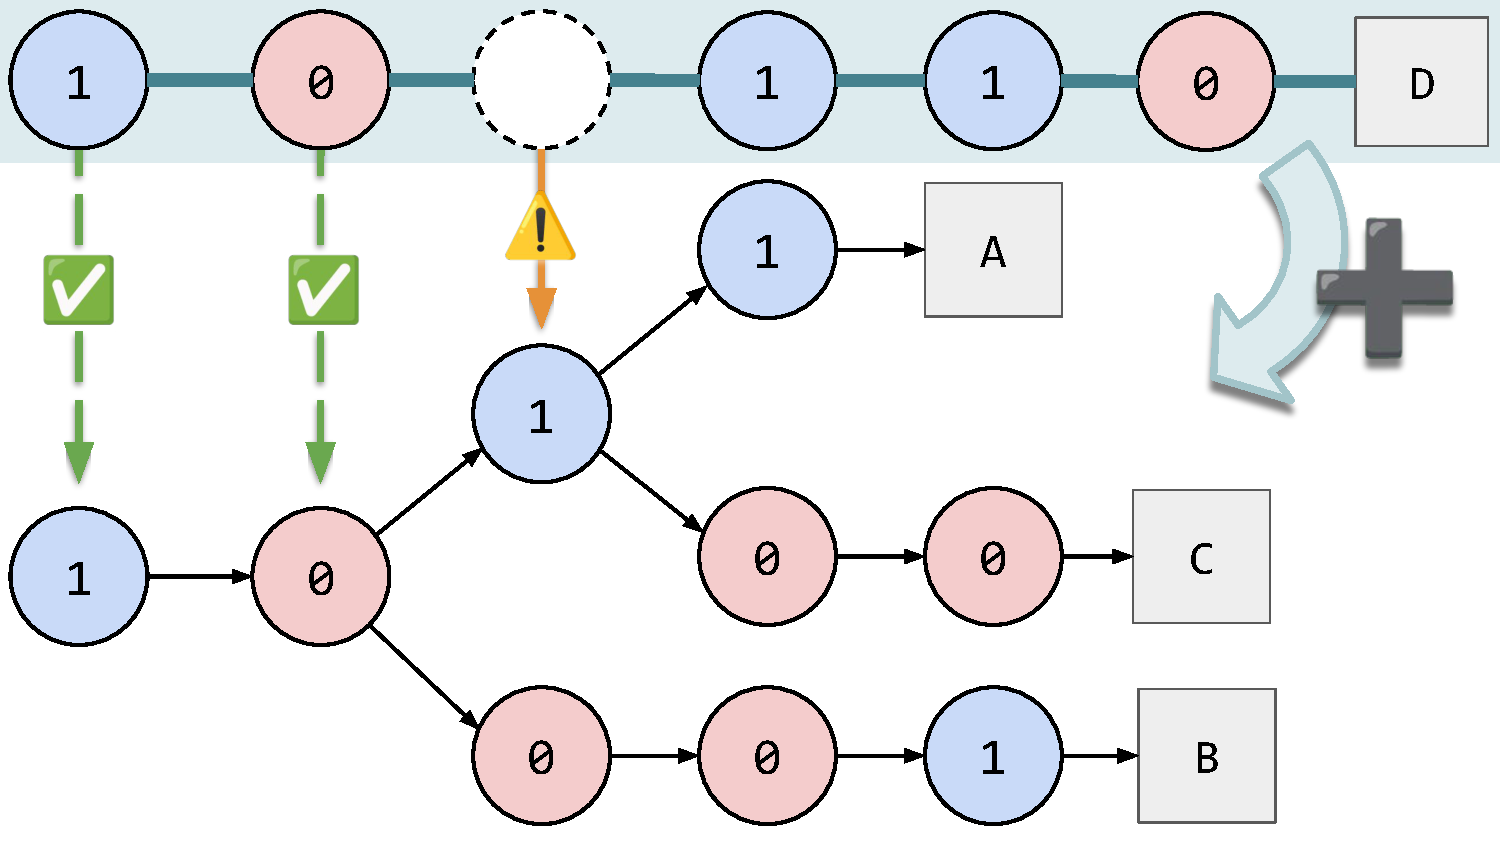
\includegraphics[width=\linewidth]{img/shortcut-algo-diagram-1}
  \subcaption{Preparing to add $D$}
  \label{fig:shortcut-algo-diagram-1}
\end{minipage}
\begin{minipage}{0.32\linewidth}
  \centering
  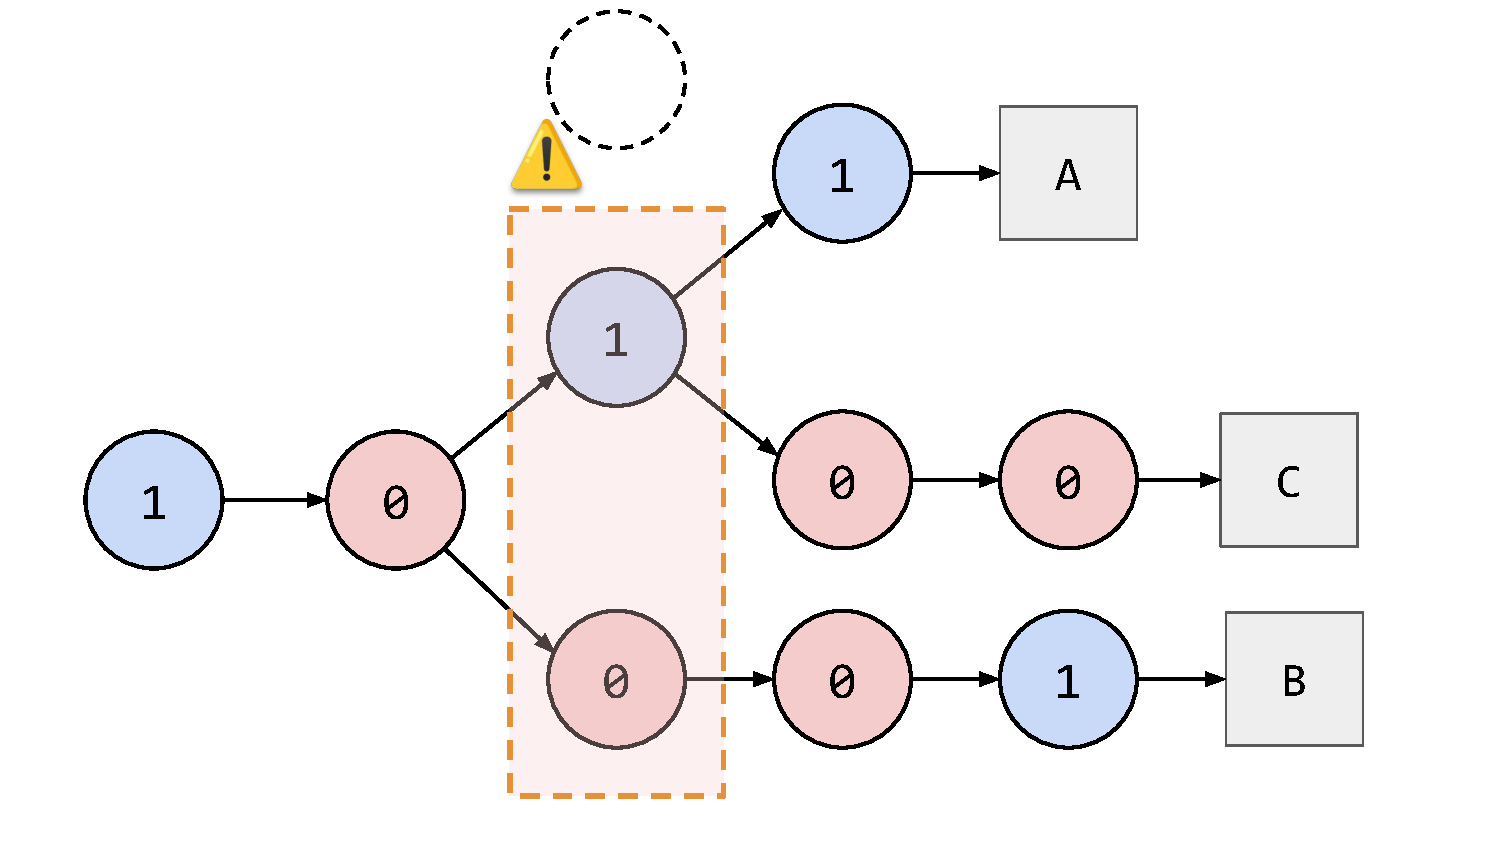
\includegraphics[width=\linewidth]{img/shortcut-algo-diagram-2}
  \subcaption{Encountering dropped marker}
  \label{fig:shortcut-algo-diagram-2}
\end{minipage}
\begin{minipage}{0.32\linewidth}
  \centering
  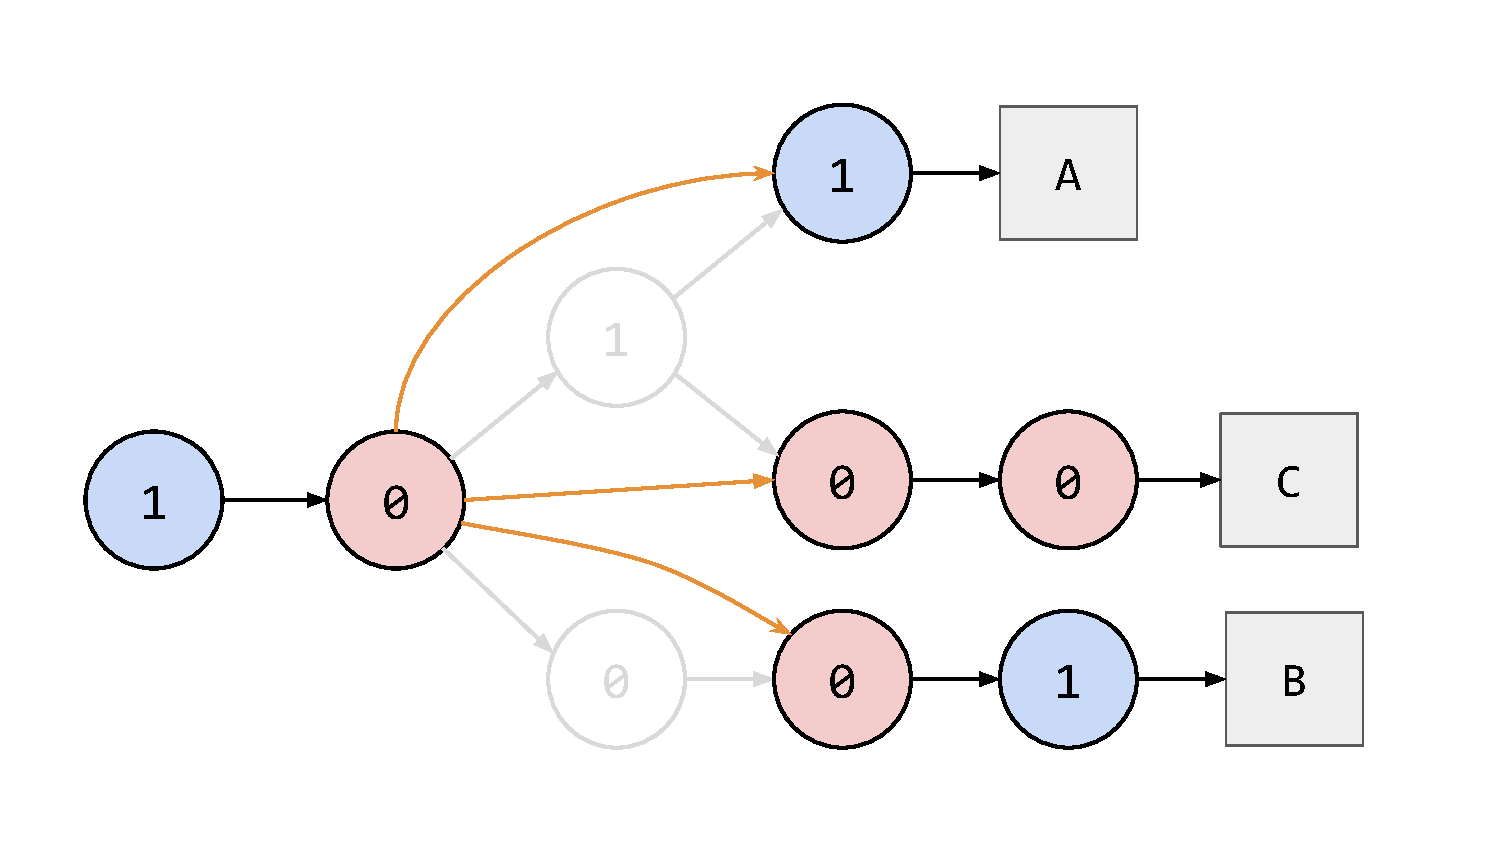
\includegraphics[width=\linewidth]{img/shortcut-algo-diagram-3}
  \subcaption{Building shortcuts}
  \label{fig:shortcut-algo-diagram-3}
\end{minipage}
\begin{minipage}{\linewidth}\par\end{minipage}
\begin{minipage}{0.32\linewidth}
  \centering
  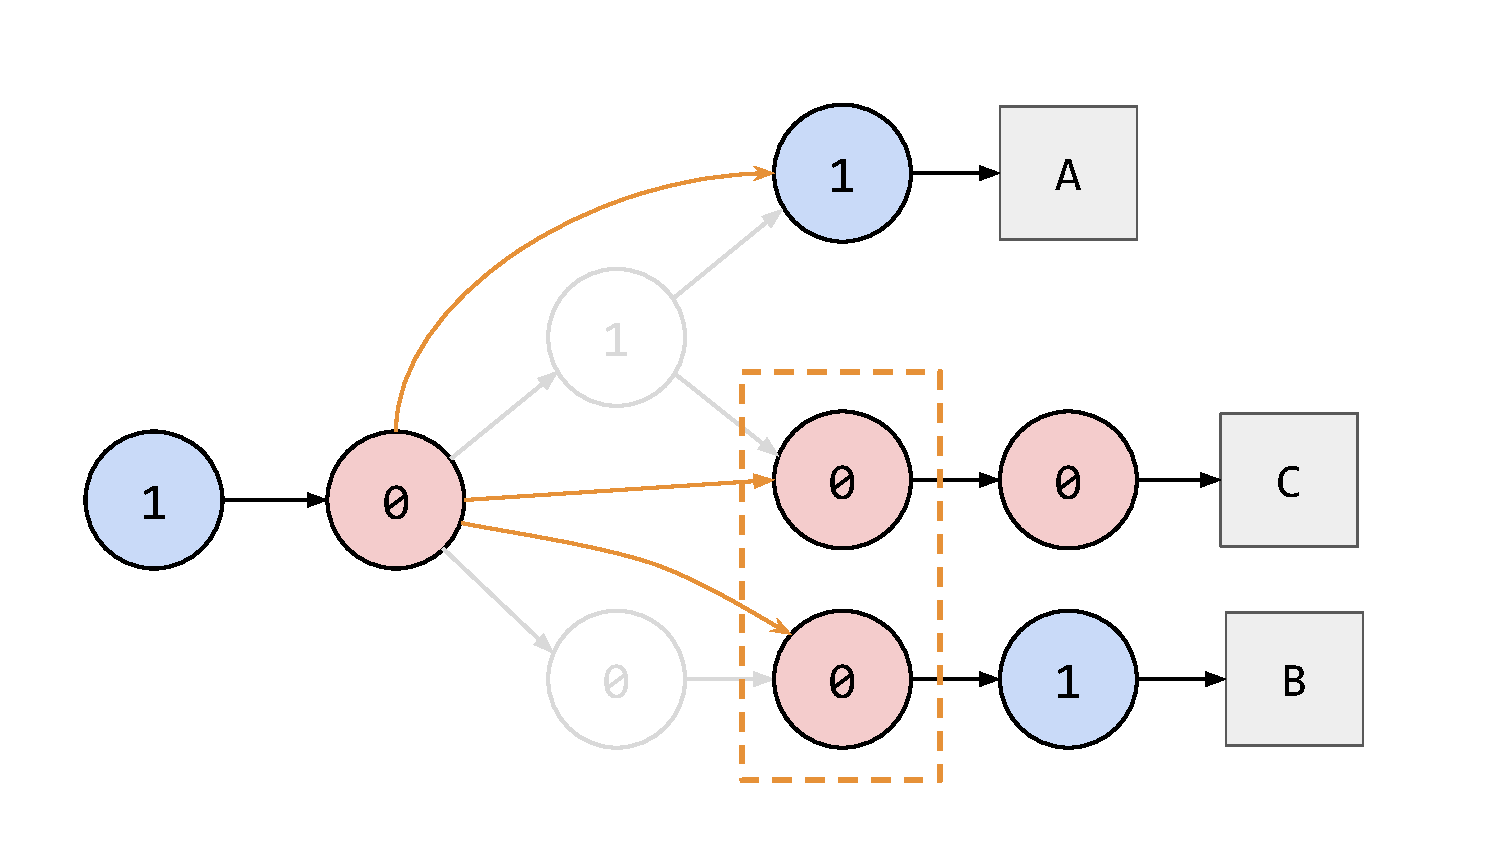
\includegraphics[width=\linewidth]{img/shortcut-algo-diagram-4}
  \subcaption{Indistinguishable nodes}
  \label{fig:shortcut-algo-diagram-4}
\end{minipage}
\begin{minipage}{0.32\linewidth}
  \centering
  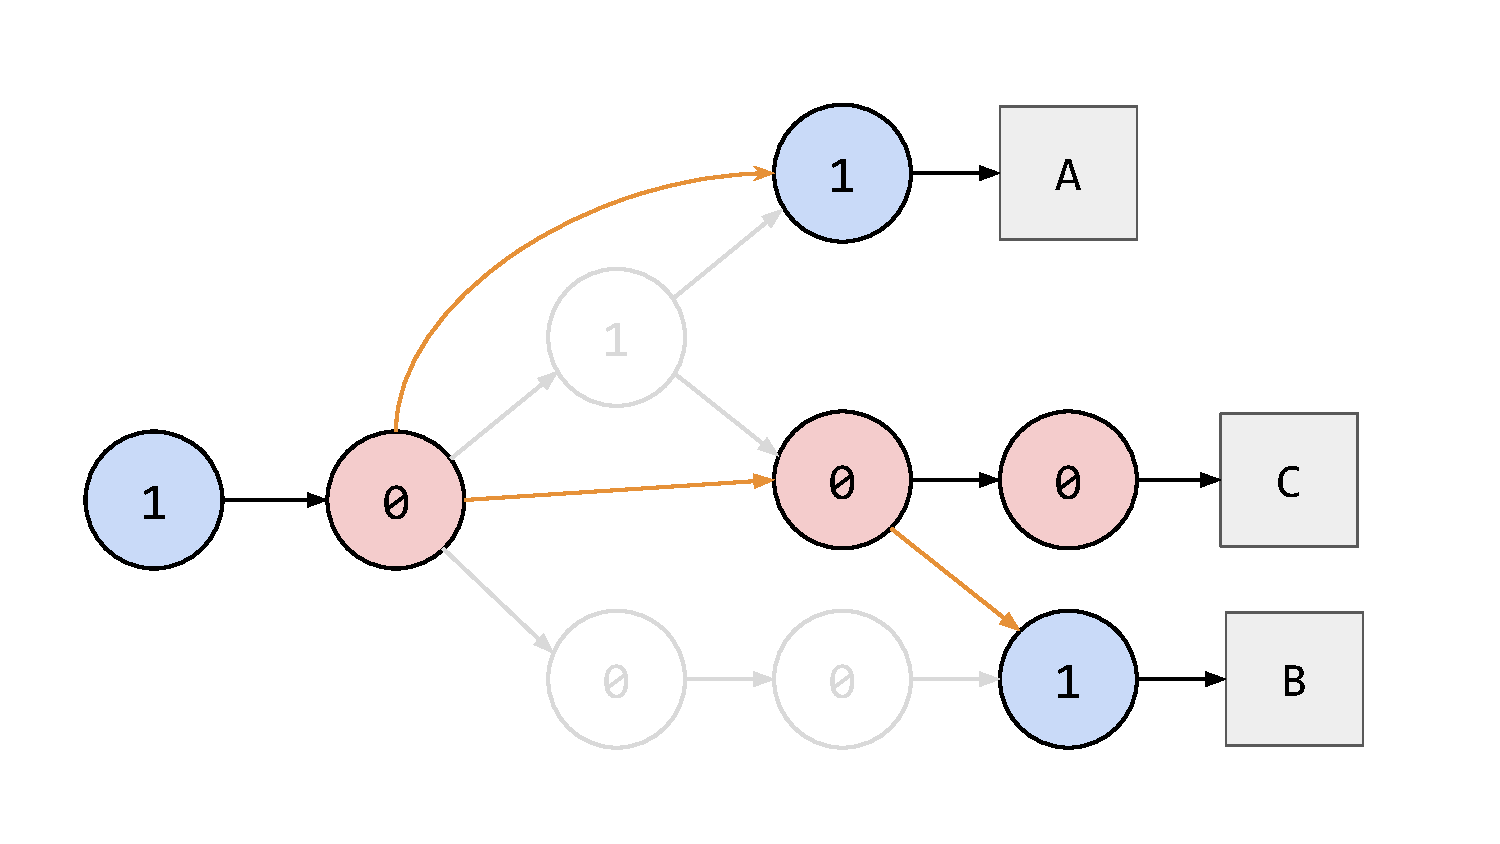
\includegraphics[width=\linewidth]{img/shortcut-algo-diagram-5}
  \subcaption{Collapsing redundant shortcuts}
  \label{fig:shortcut-algo-diagram-5}
\end{minipage}
\begin{minipage}{0.32\linewidth}
  \centering
  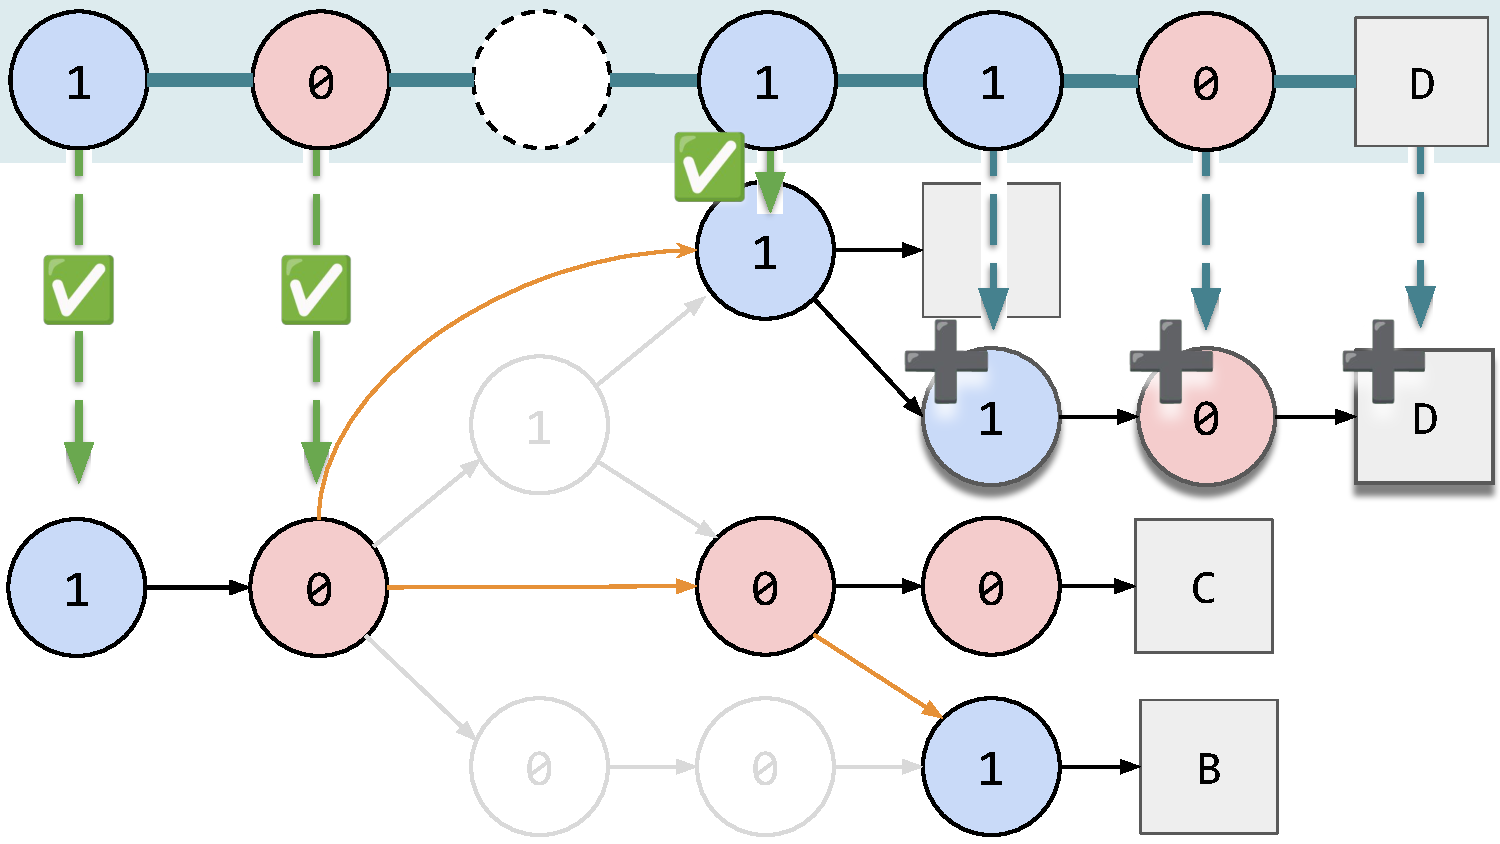
\includegraphics[width=\linewidth]{img/shortcut-algo-diagram-6}
  \subcaption{Organism $D$ added}
  \label{fig:shortcut-algo-diagram-6}
\end{minipage}
\end{minipage}
\begin{minipage}{0.24\linewidth}
\caption{%
\textbf{Trie-consolidation procedure for proposed shortcut algorithm.}
\small
A dropped hereditary marker is encountered while extending trie with genome $D$ (panel \ref{fig:shortcut-algo-diagram-2}).
All subsequent-added genomes will also have dropped markers at this position, so corresponding trie nodes may be bypassed by ``shortcut'' connections (panel \ref{fig:shortcut-algo-diagram-3}).
Note that bypassed trie structure is retained (``grayed-out'' nodes), so corresponding phylogenetic structure remains when reconstruction is finalized.
In a final step, shortcuts leading to identical nodes are further consolidated (panels \ref{fig:shortcut-algo-diagram-4} and \ref{fig:shortcut-algo-diagram-5}).
}
\label{fig:algo-diagram}
\end{minipage}
\vspace{-1.5em}
\end{figure*}


However, this process may result in some nodes in the previous level having duplicate children in the next level. This can be resolved by essentially `merging' the duplicates by choosing one to keep and creating shortcuts from the kept one to the children of the removed one (see steps 3-4 in Figure~\ref{fig:algo-diagram}). Now, adding any organisms that are missing data from the removed level becomes trivial, as the algorithm can use the newly created shortcuts as if they are part the tree itself, skipping the missing information. The key savings lie in the fact that any subsequent organisms will also be able to use these shortcuts to traverse the tree much more quickly. Additionally, since we don't exactly delete the old information (as represented by the gray nodes in Figure~\ref{fig:algo-diagram}), we preserve the accuracy and granularity of the old approach. See Algorithm~\reg{alg:consolidation} to see psuedocode for this algorithm.

\begin{algorithm}[h]
  \begin{algorithmic}[1]
  \small{
    \Function{ConsolidateTree}{tree $T$, node $n$, rank $r$}
      \State $S \gets \{c \in \operatorname{descendants}(n) : \operatorname{rank}(c) \ge r \land  \operatorname{rank}(\operatorname{parent}(c)) < r\}$ 
      \For{$c$ in $S$} 
        \textsc{BuildShortcut}($T$, $n$, $c$)
      \EndFor
      \For{each subset of duplicate\footnotemark nodes $S' \subseteq S$}
        \State $c^* \gets$ an arbitrary element in $S'$ 
        \For{$c' \in S \setminus \{c^*\}$}
          \For{$c$ in $\operatorname{children}(c)$} 
            \State \textsc{BuildShortcut}($T$, $c^*$, $c$)
          \EndFor
          \State \textsc{RemoveShortcut}($T$, $n$, $c'$)
        \EndFor
      \EndFor 
    \EndFunction
    \Function{BuildShortcut}{tree $T$, node $n$, node $c$}
      \State $\operatorname{edges}(T) \gets \operatorname{edges}(T) \cup \{(n, c)\}$
      \State $\operatorname{edges}(T)[(n, c)]\text{.is\_shortcut} \gets \textsc{True}$
    \EndFunction
    \Function{RemoveShortcut}{tree $T$, node $n$, node $c$}
        \State $\operatorname{edges}(T) \gets \operatorname{edges}(T) \setminus \{(n, c)\}$
    \EndFunction
  }
  \end{algorithmic}
  \caption{\textbf{The consolidation step of the shortcut table algorithm.} \small Builds shortcuts for a given node $n$ and collapses duplicate children caused by those shortcuts. Note that \vspace{-1.5em}}
  \label{alg:consolidation}
\end{algorithm}
\footnotetext{nodes $x$ and $y$ are duplicates iff $\operatorname{rank}(x) = \operatorname{rank}(y)$ and $\operatorname{differentia}(x) = \operatorname{differentia}(y)$}

This updated algorithm is implemented in the \texttt{hstrat} Python package \citep{moreno2024hstrat} as \texttt{build\_tree\_searchtable(\_cpp)?}. As the name suggests, it uses a table of records to represent a tree, being nearly equivalent in structure but being more cache-friendly. The shortcuts are implemented by maintaining two sets of information about ancestors, siblings, and children -- one set holding the original information and the other set holding information for the most recent shortcuts created. The latter is used whenever traversing the tree, while the former is used to preserve information. To start, these sets have the same data, but upon the creation of shortcuts, the shortcut set is updated; note that this can happen multiple times, as levels that already have shortcuts can later be removed as well.

\subsection{Accuracy}

We shall demonstrate the accuracy of this algorithm by providing a proof overview of how it is equivalent to the old algorithm (and assuming the old algorithm is a `good' reconstruction algorithm). Consider adding some organism $o$ to the reconstructed tree $T$, which follows exactly one of the following cases: there is no missing information (i.e. $\forall (r, d) \in o\ r = \operatorname{rank}(\operatorname{children}(n))$, where $n$ is the current node throughout iteration), or there is. The case where there is no missing information is trivial -- the only difference between the original and new algorithm lies when there is missing information, the absence of which rendering them the same. 

Therefore, consider analyzing data at rank $r'$ and having some missing information at rank $r < r'$ (which is also the rank of the node $n$'s children). We know that the old algorithm selects the child (possibly (great)grandchild, depending on if there is even more missing information) $n'$ of $n$ that leads to the longest successive path of matching differentiae. Additionally, note that $\operatorname{rank}(\operatorname{children}(n')) = r'$, meaning $n'$ will become the new current node $n$ in the old algorithm. Suppose there is a child of $n'$ with a differntia equal to $d$ (otherwise, the choice is $n'$ is meaningless as there would be no longest matching path). The old algorithm, treating $n'$ as $n$, will detect this child and make it the new current node, essentially continuing along the path. 

Looking at the new algorithm, notice that this node $n'$ would have actually been hidden through consolidation, with shortcuts build around it from $n$ to its children. However, notice that we had assumed that there was indeed a child of $n'$ with a differentia equal to $d$; since this is also a child of $n$ through the shortcuts, it will be chosen by the new algorithm to be the new current node $n$, also continuing along the path. We also address the fact that, in the new algorithm, this child may have more children than in the old algorithm, due to the collapse step merging it with another descendant of $n$. However, this is not a problem, as the original `longest path' is still preserved (and is still better than any paths along the children of the other descendant). In conclusion, the consolidated algorithm will make the same decisions as the original algorithm, meaning they are essentially equivalent. \qed

\subsection{Performance Benchmarks}

TODO.

\subsection{Software and Data Availability} \label{sec:materials}

Supporting software and executable notebooks for this work are available via Zenodo at TODO \citep{moreno2024hsurf}.
DStream algorithm implementations are also published on PyPI in the \texttt{downstream} Python package, where we plan to conduct longer-term, end-user-facing development and maintenance \citep{moreno2024downstream}.
All accompanying materials are provided open-source under the MIT License.

This project benefited significantly from open-source scientific software \citep{2020SciPy-NMeth,harris2020array,reback2020pandas,mckinney-proc-scipy-2010,waskom2021seaborn,hunter2007matplotlib,moreno2023teeplot}.
